%%\documentclass{beamer}
%%\documentclass[handout,usenames,dvipsnames]{beamer}
\documentclass[usenames,dvipsnames]{beamer}
\usepackage[numbers,totalnumber,sidebarshades]{beamerthemeUppsala}

\usepackage[utf8]{inputenc}
\usepackage[T1]{fontenc}
\usepackage{xcolor}
\usepackage{import}
\usepackage{listings}
\usepackage{hyperref}

%%%%%% Bibliograpy as footnotes %%%%
\usepackage{graphicx}
\usepackage[giveninits=true]{biblatex}
%\bibliography{../1DL010-21}

\graphicspath{{imgs/}}

\usepackage{pgfpages}
%\setbeameroption{show notes on second screen}
\setbeamertemplate{note page}{\insertnote}

%%\setbeamercovered{transparent}

\usepackage{xspace}
\usepackage{stmaryrd}
\usepackage{comment}

\newcommand{\tc}{\textcolor}
\newcommand{\largeskip}{\vspace{1cm}}
\newcommand{\nat}{\ensuremath{\mathbb{N}}}
\newcommand{\ra}{\ensuremath{\rightarrow}}

\newcommand{\states}{\ensuremath{S}}
\newcommand{\sts}{\ensuremath{s}}
\newcommand{\inits}{\ensuremath{s_I}}
\newcommand{\isg}{\ensuremath{g}}
\newcommand{\actions}{\ensuremath{A}}
\newcommand{\actf}{\ensuremath{\mathsf{av}}}
\newcommand{\acta}{\ensuremath{a}}
\newcommand{\trf}{\ensuremath{\delta}}
\newcommand{\costf}{\ensuremath{c}}
\newcommand{\utilf}{\ensuremath{u}}

\newcommand{\players}{\ensuremath{P}}
\newcommand{\maxp}{\ensuremath{\text{\textsc{max}}}}
\newcommand{\minp}{\ensuremath{\text{\textsc{min}}}}

\newcommand{\pts}{\ensuremath{PTS}}
\newcommand{\gts}{\ensuremath{GTS}}

\newcommand{\bstates}{\ensuremath{Q}}
\newcommand{\stb}{\ensuremath{q}}
\newcommand{\isf}{\ensuremath{f}}

\newcommand{\set}[1]{\ensuremath{ \{ #1 \}}}
\newcommand{\ol}{\ensuremath{\overline}}

\newcommand{\turnf}{\ensuremath{t}}

%%\newcommand{\land}{\wedge}
%%\newcommand{\lor}{\wee}
\newcommand{\lra}{\leftrightarrow}
\newcommand{\propl}{\mathcal{L}_p}

\newcommand{\M}{\mathcal{M}}
\newcommand{\lang}{\mathcal{L}}
\newcommand{\sat}{\ensuremath{\mathsf{SAT}}\xspace}
\newcommand{\limp}{\ensuremath{\mathsf{LIMP}}\xspace}

\newcommand{\const}{\boldsymbol}
\newcommand{\terms}{\mathit{TM}}
\newcommand{\term}{t}
\newcommand{\atoms}{ATOM}
\newcommand{\forms}{FORM}
\newcommand{\fv}{FV}
\newcommand{\struct}{\mathcal{S}}
\newcommand{\dom}{\Delta}

\newcommand{\intf}{I}

\newcommand{\te}{\ensuremath{\bar{v}}}
\newcommand{\va}{\ensuremath{v}}

\newcommand{\quant}{\ensuremath{\mathcal{Q}}}

\newcommand{\reals}{\ensuremath{\mathbb{R}}}

\newcommand{\hsig}{\ensuremath{h_{sig}}}
\newcommand{\logl}{\ensuremath{L_{\ell \ell}}}

\newcommand{\vechsig}{\ensuremath{\bar{h}_{sig}}}


%%%%%%%%%%%% Fabio ML %%%%%%%%%%%%%%%%%%
\def\riga{\vskip 1\baselineskip \noindent}
\newcommand{\bi}{\begin{itemize}\setlength{\itemsep}{-0.1em}}
\newcommand{\ei}{\end{itemize}}
\newcommand{\be}{\begin{enumerate}}
\newcommand{\ee}{\end{enumerate}}
%%%%%%%%%%%%%%%%%%%%%%%%%%%%%%%%%%%



%%%%%%%%%%% FNN %%%%%%%%%%%%%%%%%%%%
\newcommand{\nnw}[2]{w^{(#1)}_{#2}}
\newcommand{\nnW}[1]{\pmb{W}^{(#1)}}
\newcommand{\nna}[2]{a^{(#1)}_{#2}}
\newcommand{\nnA}[1]{\pmb{a}^{(#1)}}
\newcommand{\nnz}[2]{z^{(#1)}_{#2}}
\newcommand{\nnZ}[1]{\pmb{z}^{(#1)}}
\newcommand{\nnh}{\pmb{h}}
\newcommand{\nndelta}[2]{\delta^{(#1)}_{#2}}
\newcommand{\nnDELTA}[2]{\Delta^{(#1)}_{#2}}
\newcommand{\nnDelta}[1]{\pmb{\delta}^{(#1)}}
\newcommand{\nnDDELTA}[1]{\pmb{\Delta}^{(#1)}}


%%%%%%%%%%%%%%%%%%%%%%%%%%%%%%%%%%






%%%%%%%%%%%%%%%%%%%%%%%%%%%%%%%%%%%%%%%%
\title{1DT109 - Accelerating systems with FPGAs}
\subtitle{Expressive power of neural networks}

\author[R.\ De Masellis]{Riccardo De Masellis}
\date[]{\today}
\institute[uu.se]{Uppsala University}

\begin{document}

\begin{frame}[plain]
  \titlepage
\end{frame}
%%%%%%%%%%%%%%%%%%%%%%%%%%%%%%%%%%%%%%%
%\section{Universality of Neural Networks}
%\frame{
%\setbeamercovered{transparent}
%\tableofcontents[currentsection,
%        currentsubsection,
%        subsectionstyle=shaded]
%}
%%%%%%%%%%%%%%%%%%%%%%%%%%%%%%%%%%%%%%%
\begin{frame}
  \frametitle{On computing functions}


\begin{ntblock}
\centering
A neural network with one hidden layer can \tc{red}{approximate} (to any desired precision) any \tc{red}{continuous} function with any number of inputs and outputs (Cybenko '89).
\end{ntblock}

\pause

%\begin{itemize}
  %\item 
  the more hidden neurons, the better the approximation (fix $\varepsilon > 0$, there exists a number of hidden neurons such that the error of the net is below $\varepsilon$ for every input).
%\end{itemize}

\vfill \pause

\begin{ntblock}
\centering
Therefore, neural networks are ``\tc{blue}{universal} computational devices''.
\end{ntblock}

\end{frame}


%%%%%%%%%%%%%%%%%%%%%%%%%%%%%%%%%%%%%%%
\begin{frame}
  \frametitle{Simple case}
  
  Let us consider a single input-single output function:
  
  \centering
  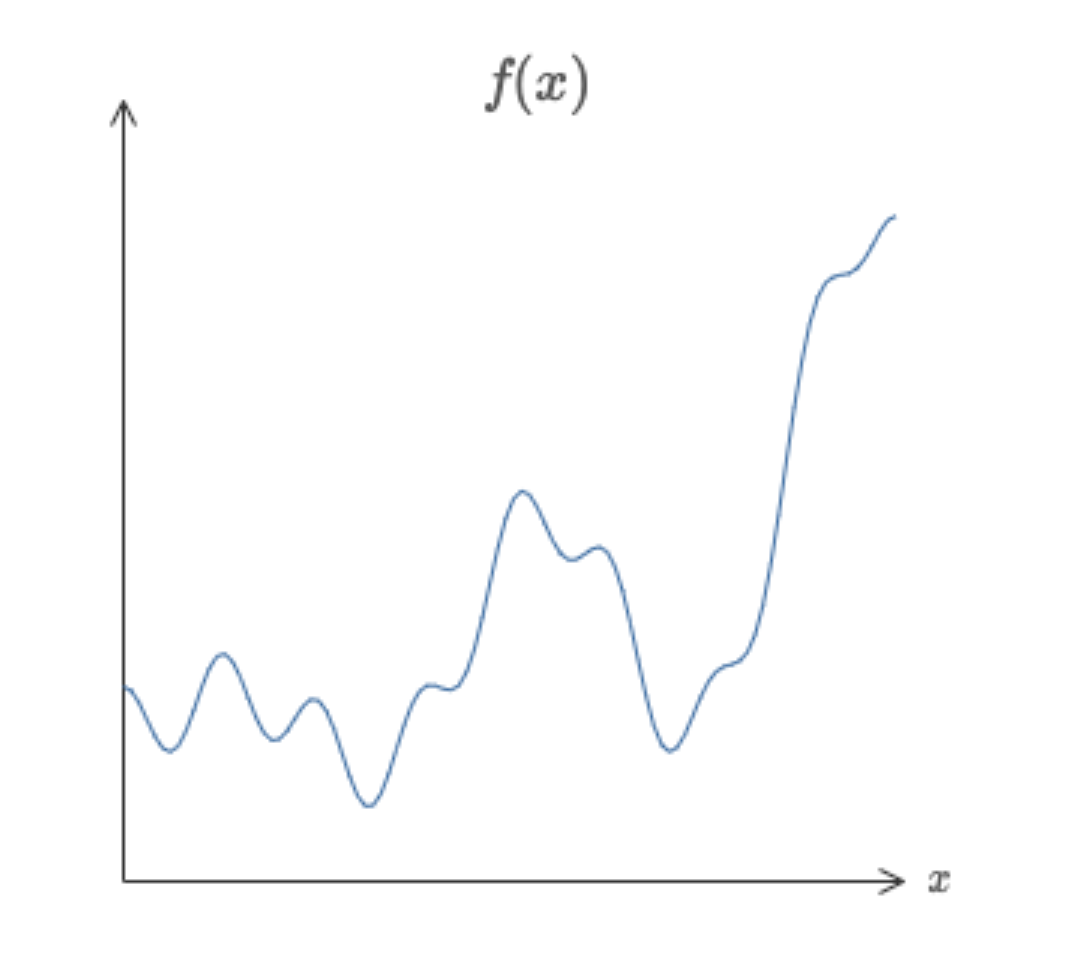
\includegraphics[scale=.3]{cont-func}
\end{frame}
%%%%%%%%%%%%%%%%%%%%%%%%%%%%%%%%%%%%%%%

\begin{frame}
  \frametitle{Step 1: what a single hidden neuron can compute}
  
  \begin{center}
  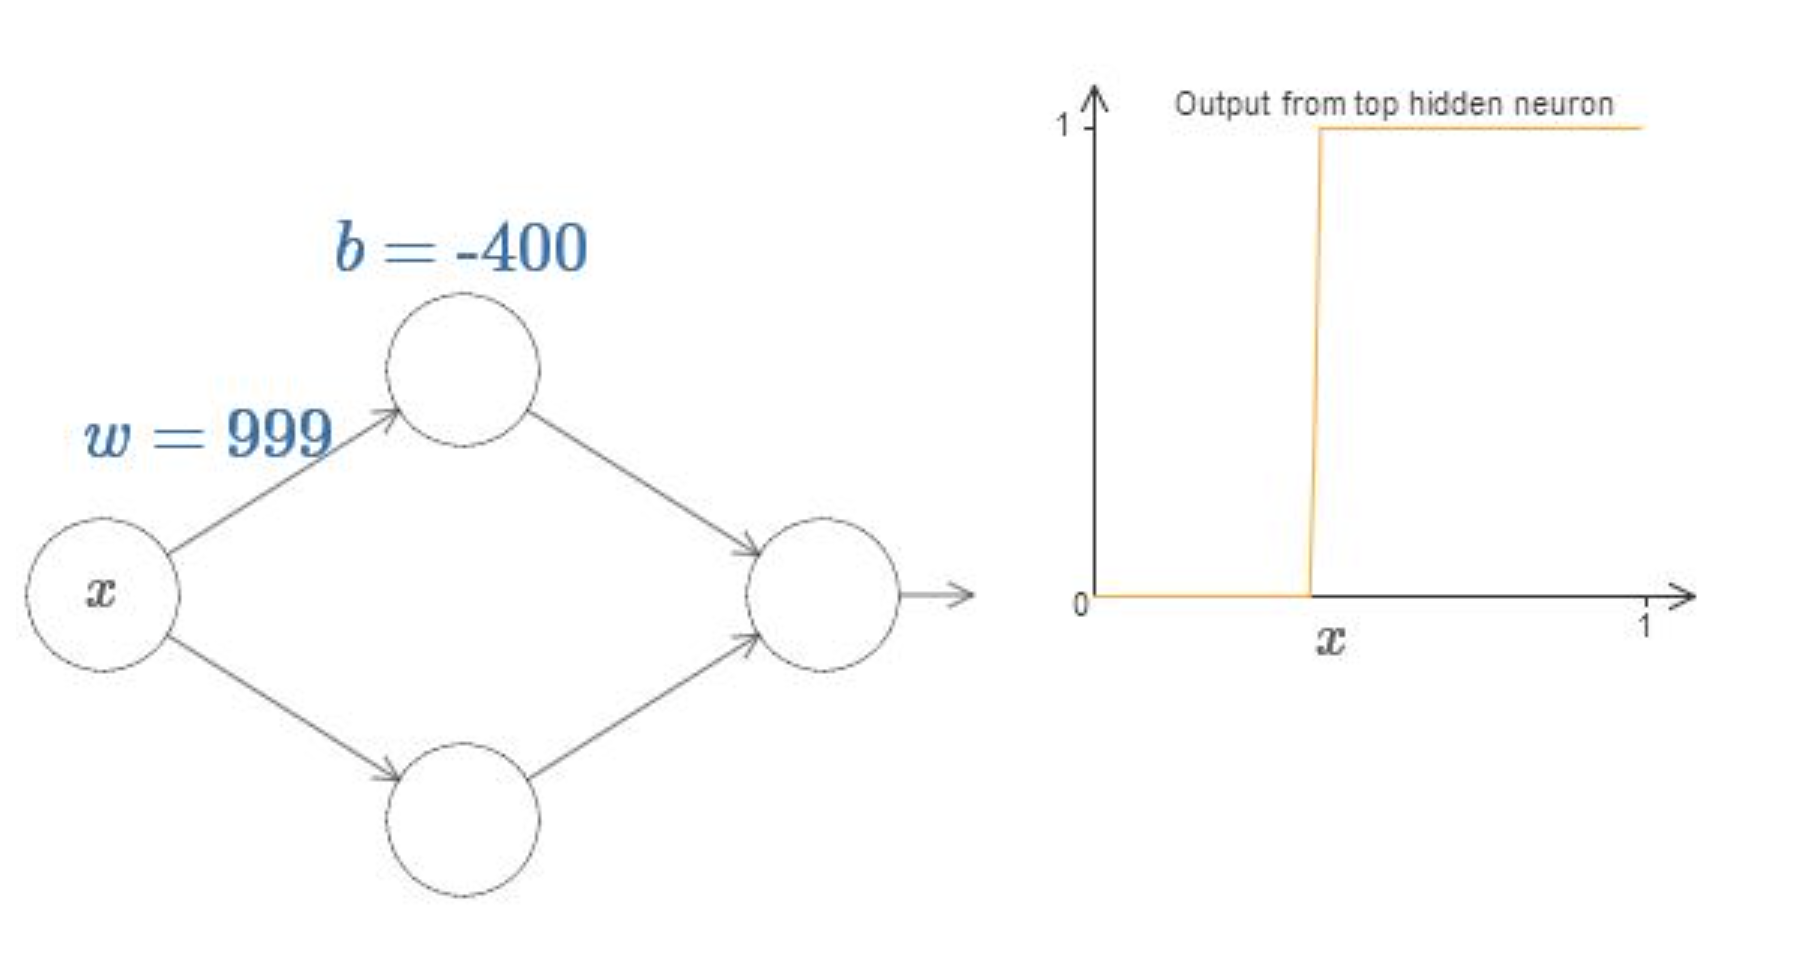
\includegraphics[scale=.3]{single-hid-neu}
  \end{center}
  
  \begin{enumerate}
  \item fix the weight $w$ to a large value;
  \item set the position by modifying the bias	 $b$.
  \end{enumerate}

  
  {\footnotesize (We use step functions as it is easier to understand their contribution to the output layer)}
  
\end{frame}

%%%%%%%%%%%%%%%%%%%%%%%%%%%%%%%%%%%%%%%
\begin{frame}
  \frametitle{Position of the step function}
  
  With large values of $w$, the position of the step is:
  
  \[s = - \frac{b}{w}\]
  
  \vfill
  
 \centering
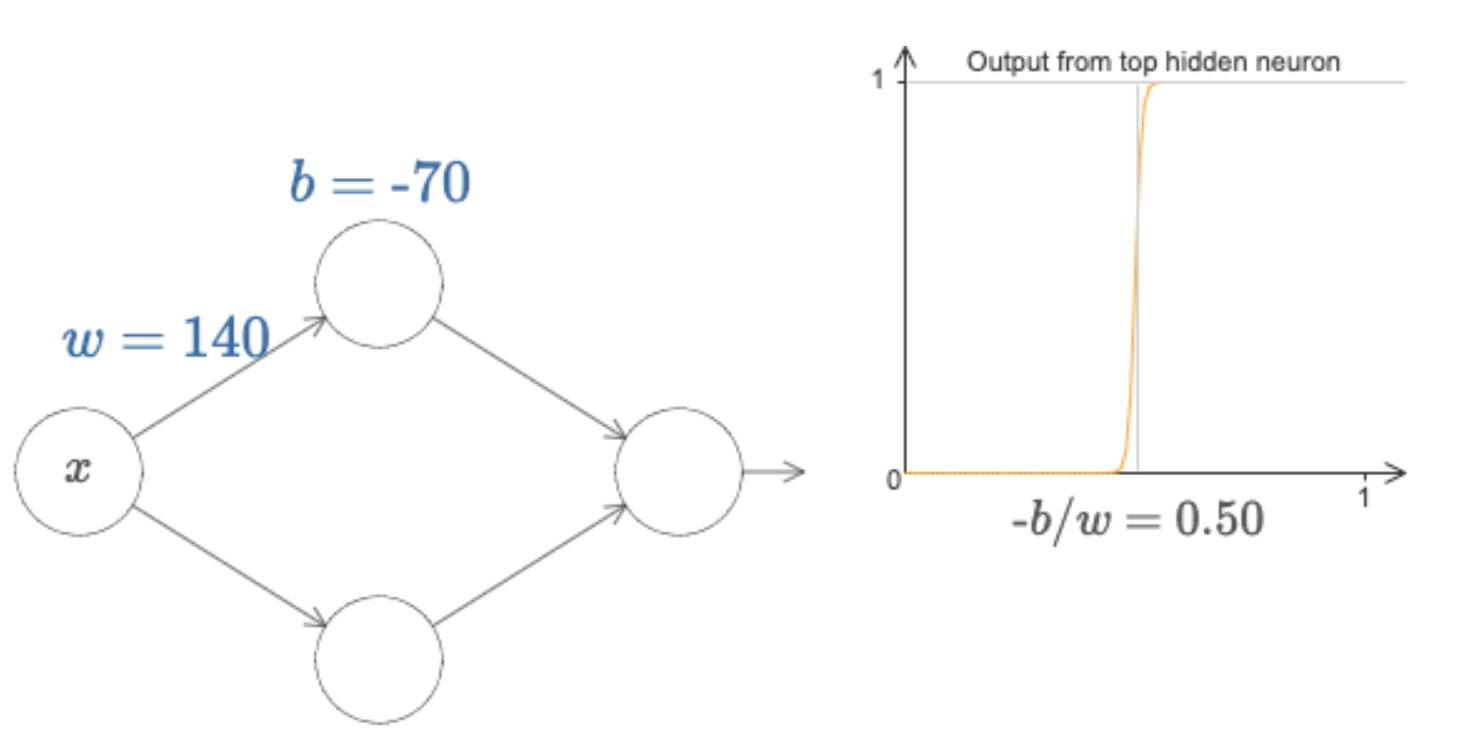
\includegraphics[scale=.35]{step-pos}

\end{frame}



%%%%%%%%%%%%%%%%%%%%%%%%%%%%%%%%%%%%%%%
\begin{frame}
  \frametitle{Step 2: adding a neuron}
  
  Let us consider the contributions of the bottom hidden neuron.
  
  \begin{center}
 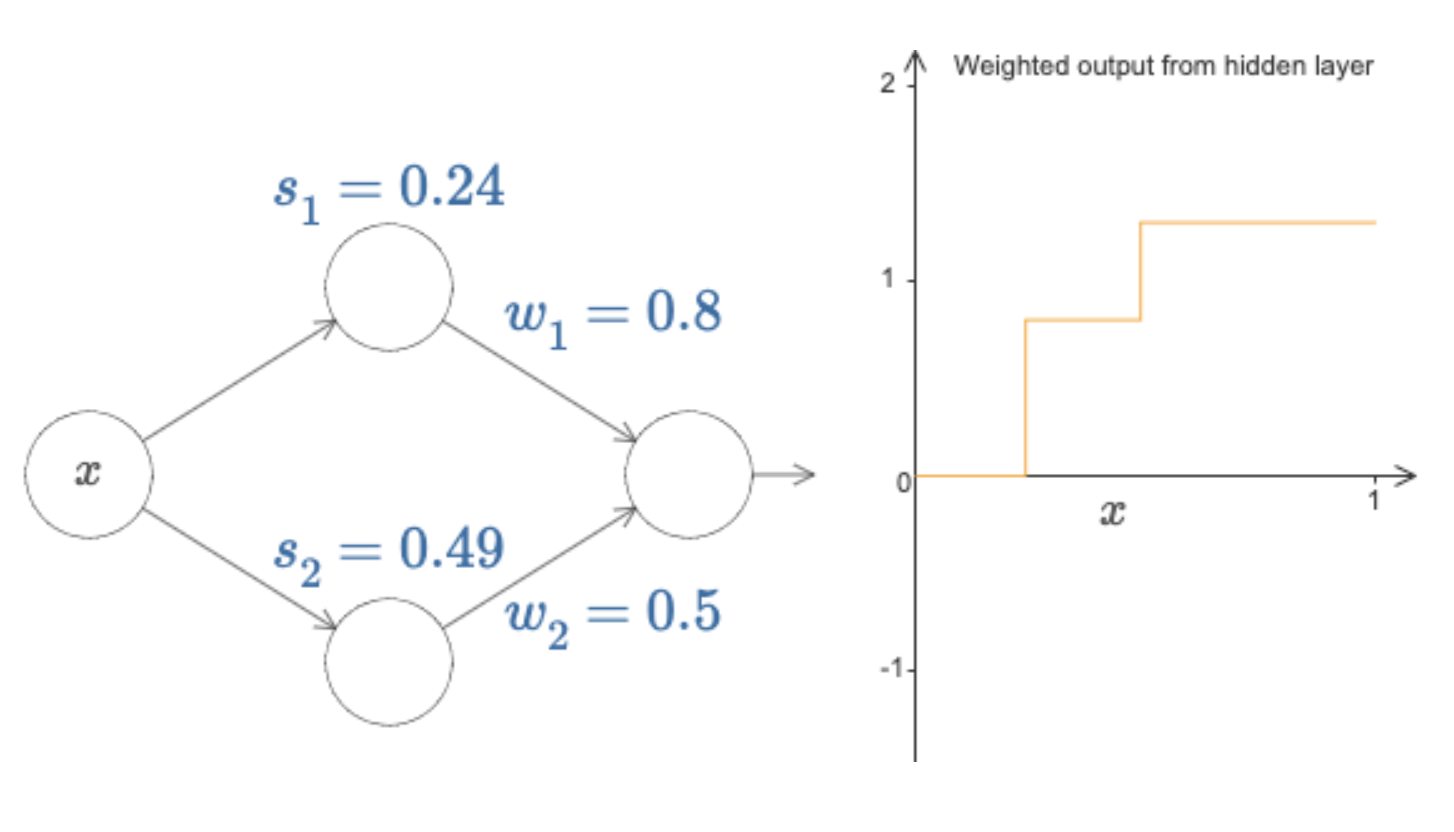
\includegraphics[scale=.30]{more-stepf} 
 \end{center}
 
 The plot is for $w_1a_1 + w_2a_2$ where $a_1$ and $a_2$ are the \emph{activations} of the top and bottom hidden neurons. This is different from the output of the net, which computes $\sigma(w_1a_1 + w_2a_2 + b)$ where $b$ is the bias of the output neuron.
  
\end{frame}

%%%%%%%%%%%%%%%%%%%%%%%%%%%%%%%%%%%%%%%
\begin{frame}
  \frametitle{Step 3: the ``bump''}
  
  By adjusting the weights of the output layer, we can obtain a ``bump'' of any height, positioned depending on $s_1$ and $s_2$.
  
  \vfill
  
  \centering
  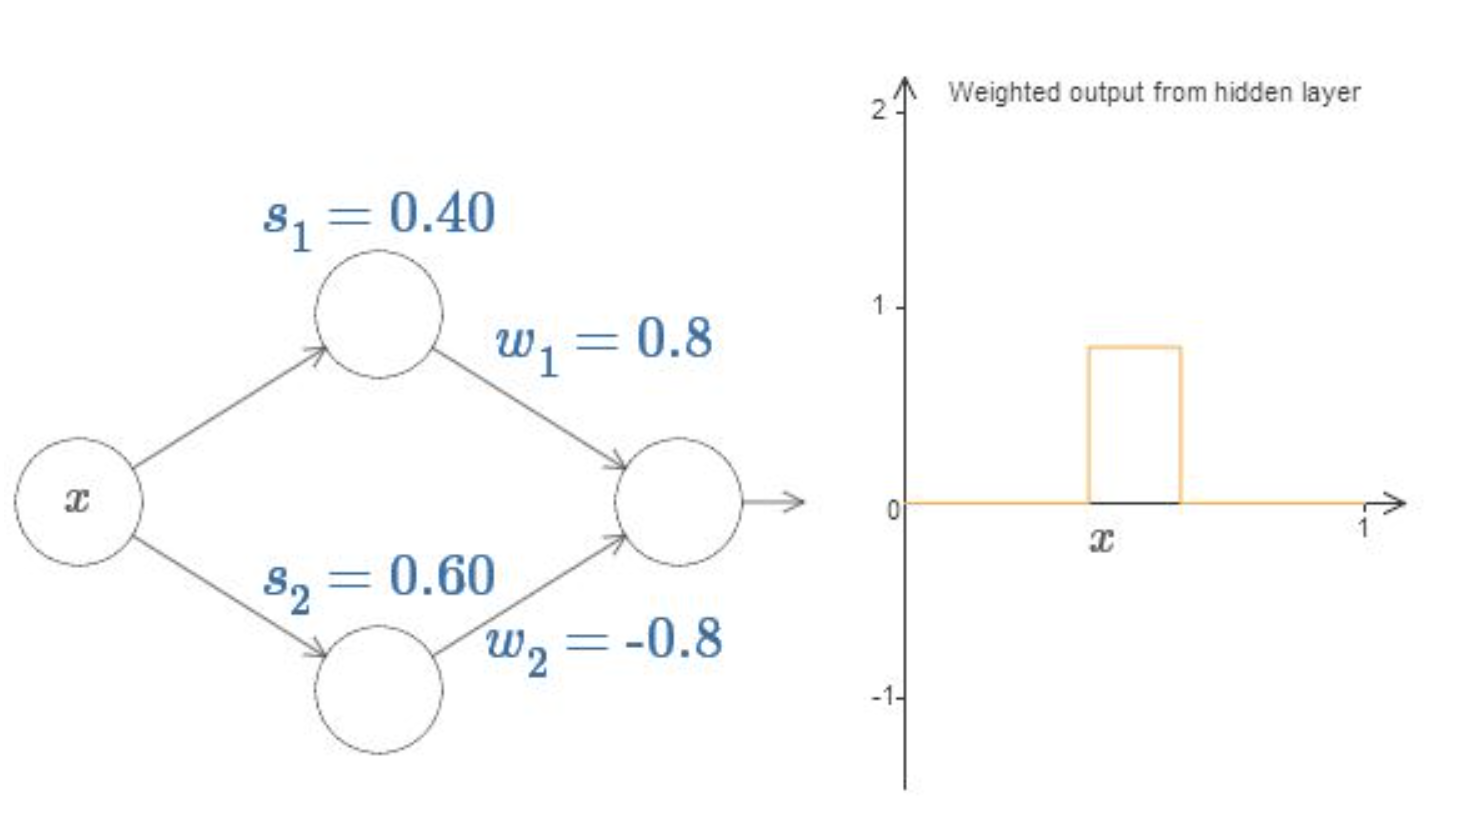
\includegraphics[scale=.35]{bump} 
  
  \vfill
  \flushleft
  To simplify notation, we can introduce parameter $h$ for the height (instead than $w_1$ and $w_2=-w_1$).
  
\end{frame}

%%%%%%%%%%%%%%%%%%%%%%%%%%%%%%%%%%%%%%%%

\begin{frame}
  \frametitle{Step 4: add pairs of hidden neurons}
  
  By adding pairs of hidden neurons, each pair ``generating'' a bump...
  
  \vfill
  
    \centering
  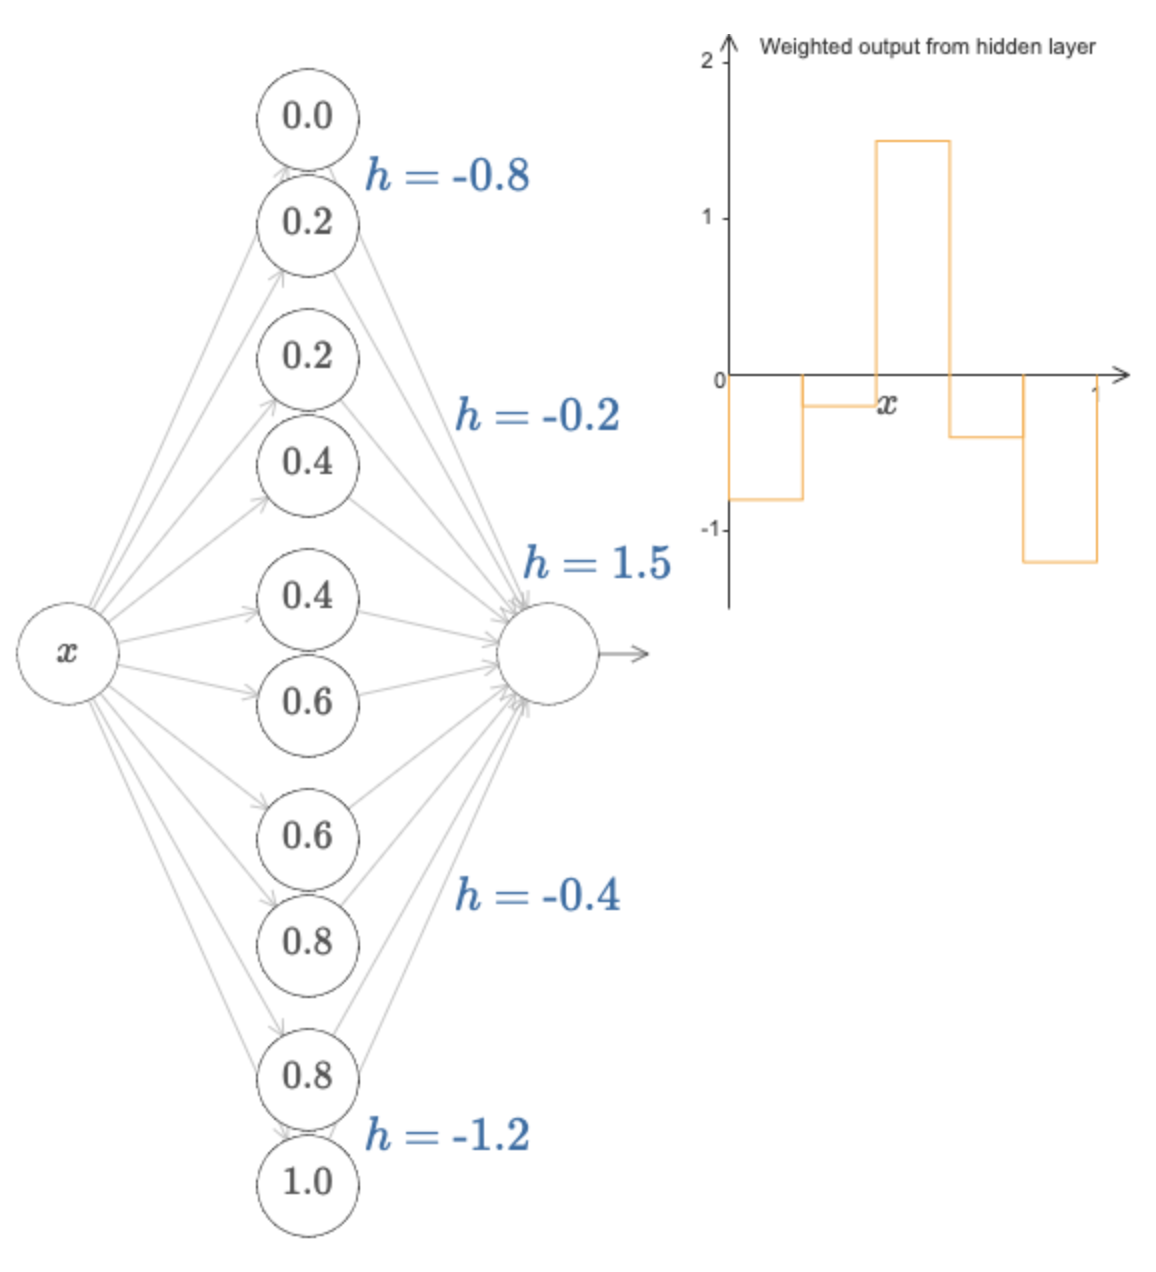
\includegraphics[scale=.35]{more-neurons} 
  
\end{frame}
%%%%%%%%%%%%%%%%%%%%%%%%%%%%%%%%%%%%%%%%%%%%%

\begin{frame}
  \frametitle{The missing step}
  
The plots so far show the weighted sum of the activation of the hidden layer, not the output of the network...

\pause

\begin{minipage}[c]{.45\textwidth}
	\centering
	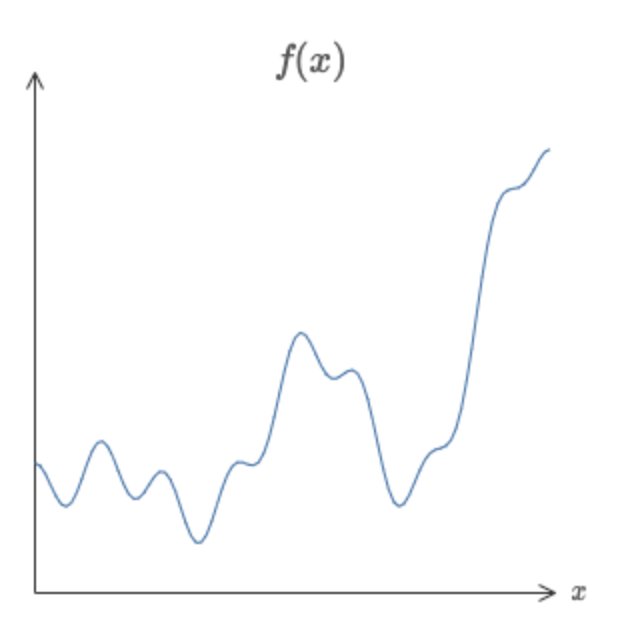
\includegraphics[scale=.3]{f} 
\end{minipage} \hfill \begin{minipage}[c]{.45\textwidth}
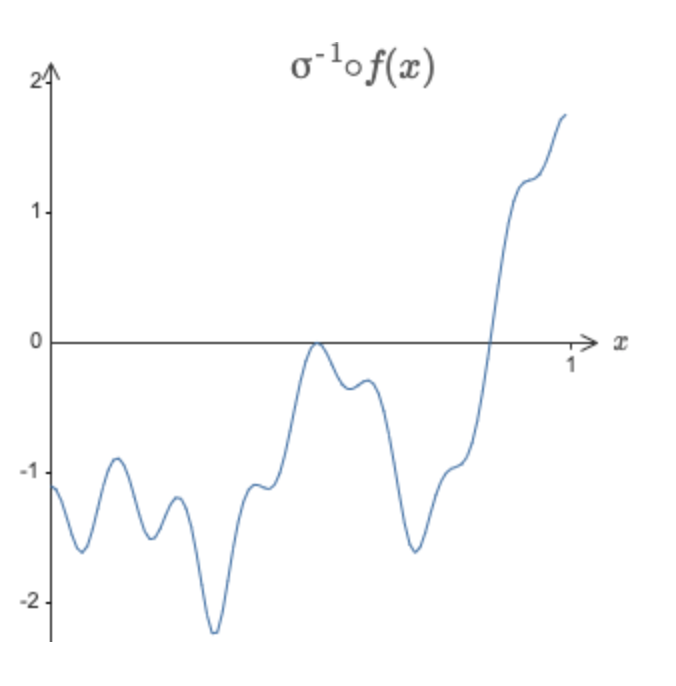
\includegraphics[scale=.3]{sigma-1f}
\end{minipage}
  
  \vfill
  
If we try to approximate $\hat{f} = \sigma^{-1}(f(x))$ with $w_1a_1 + w_2a_2 + \ldots w_na_n$ then the output of the NN is:

\[ \sigma(\hat{f}) = w_1a_1 + w_2a_2 + \ldots w_na_n \]
  
  where $\sigma^-1$ is the \tc{red}{inverse} of $\sigma$ and we set the bias of the last layer to $0$.
  
\end{frame}
%%%%%%%%%%%%%%%%%%%%%%%%%%%%%%

\begin{frame}
  \frametitle{Many input variables, single hidden neuron}
  
  Same idea but on a $n$-dimensional space.
  
  \vfill

	\centering
	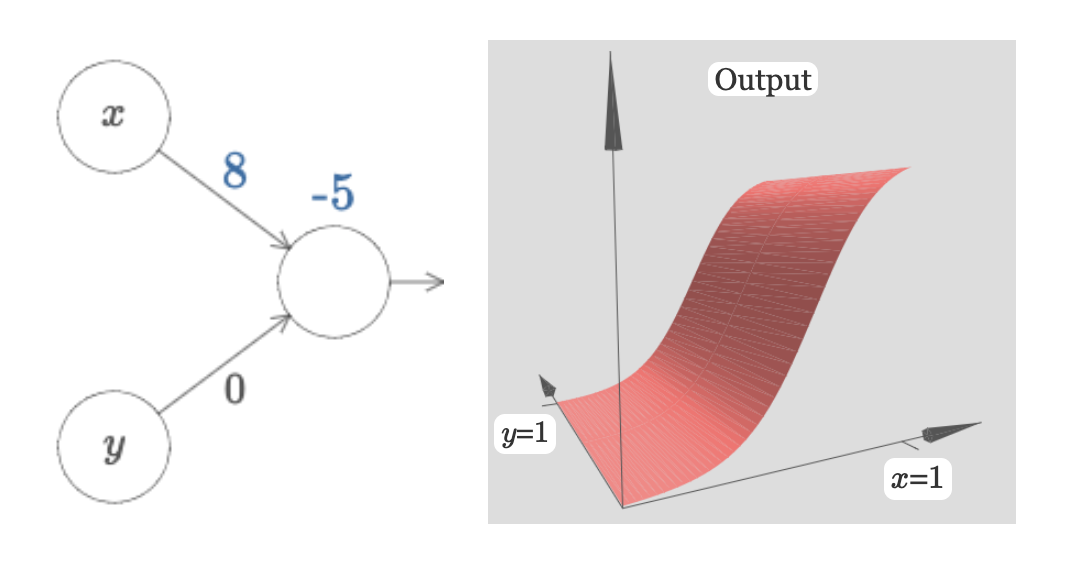
\includegraphics[scale=.35]{multi-sigmoid}

\end{frame}





%%%%%%%%%%%%%%%%%%%%%%%%%%%%%%%%%%%%%%%%%%%%%%%%%
\begin{frame}
  \frametitle{Step function in $x$ and $y$ directions}
  
    \begin{minipage}[c]{.45\textwidth}
	\centering
	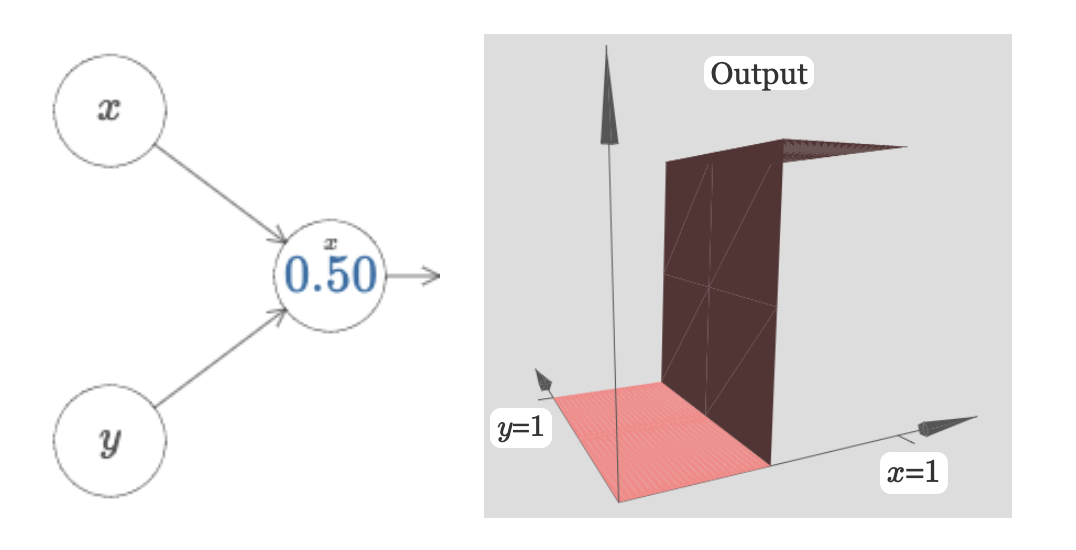
\includegraphics[scale=.3]{multi-step-x}
	\[ S_x = -\frac{b}{w_1} \text{ with } w_2=0 \]
\end{minipage} \hfill \begin{minipage}[c]{.45\textwidth}
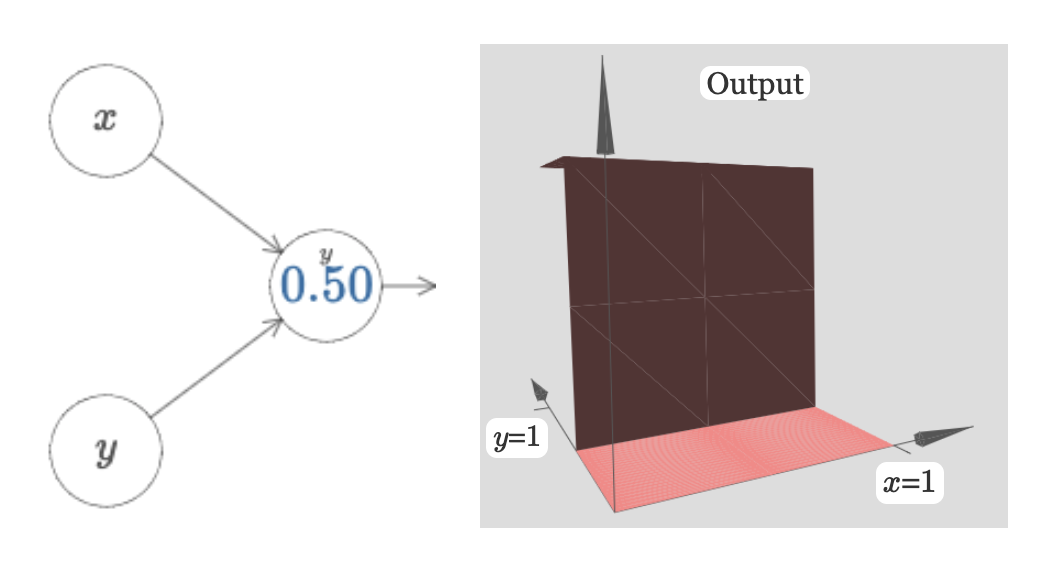
\includegraphics[scale=.3]{multi-step-y}
\[ S_y = -\frac{b}{w_2} \text{ with } w_1=0 \]
\end{minipage}
  
\end{frame}



%%%%%%%%%%%%%%%%%%%%%%%%%%%%%%%%%%%%%%%%%%%%%%

\begin{frame}
  \frametitle{Two hidden units: multi-dimensional bump}
  
  \centering
  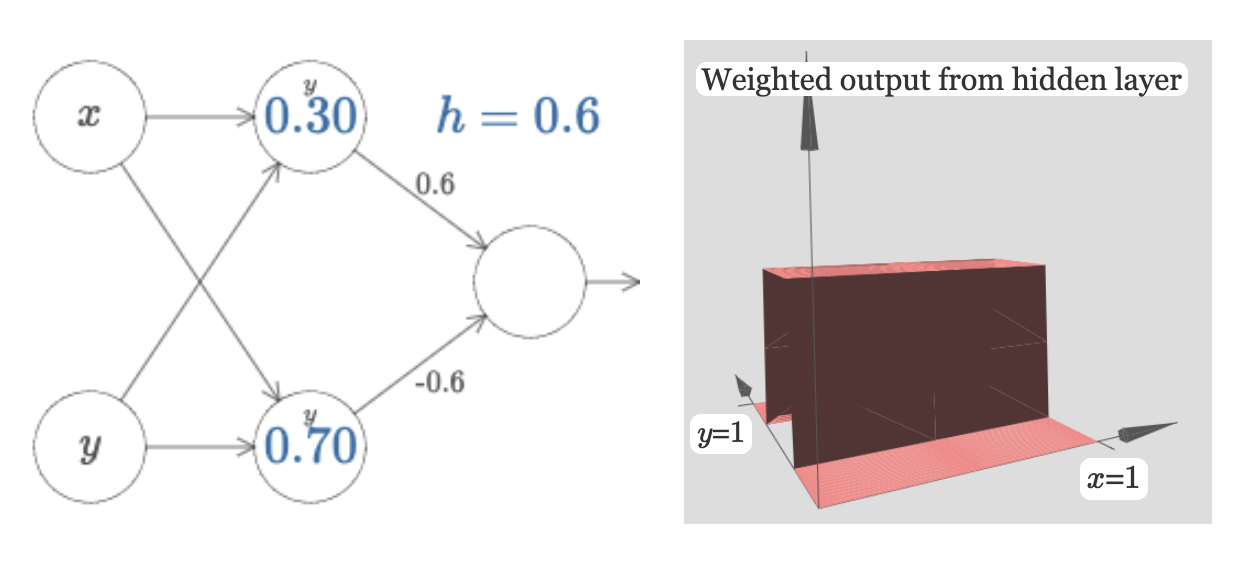
\includegraphics[scale=.4]{multi-bump}

\flushleft
where parameter $h$ is as before, and controls the height of the bump.
  
\end{frame}

%%%%%%%%%%%%%%%%%%%%%%%%%%%%%%%%%%%%%%%%

\begin{frame}
  \frametitle{More hidden neurons...}
  
  \centering
  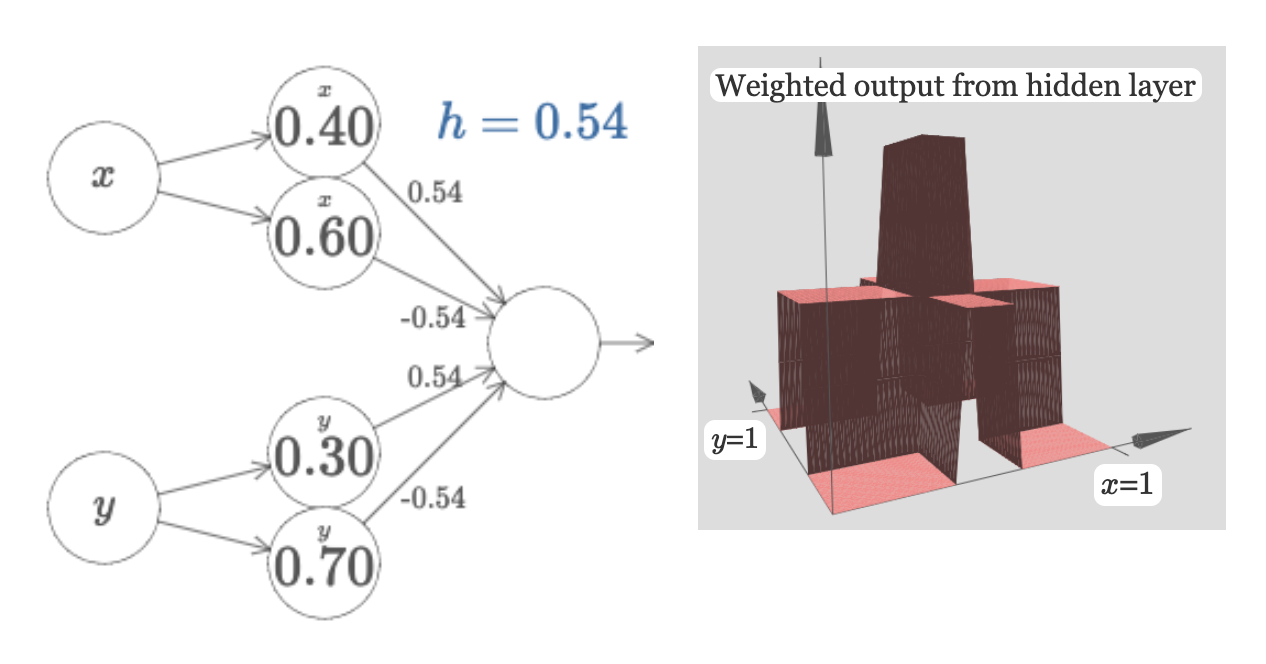
\includegraphics[scale=.4]{more-multi}
  
\end{frame}

%%%%%%%%%%%%%%%%%%%%%%%%%%%%%%%%%%%%%%%%%%%%%%%%%%

\begin{frame}
  \frametitle{Now we do need the bias on the output layer}
  
    \centering
  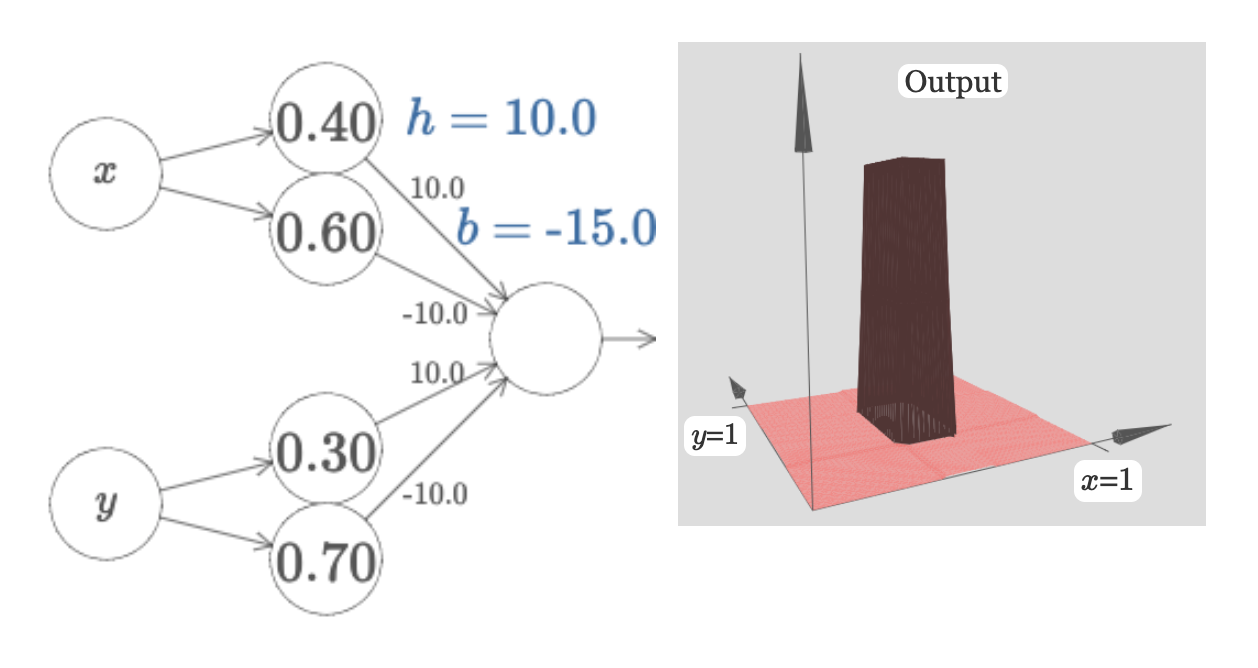
\includegraphics[scale=.4]{tower}
  
  
  Generally, $b \approx -\frac{3h}{2}$
  
\end{frame}

%%%%%%%%%%%%%%%%%%%%%%%%%%%%%%%%%%%%%%%%%%%%

\begin{frame}
  \frametitle{More towers...}
  
 \centering
  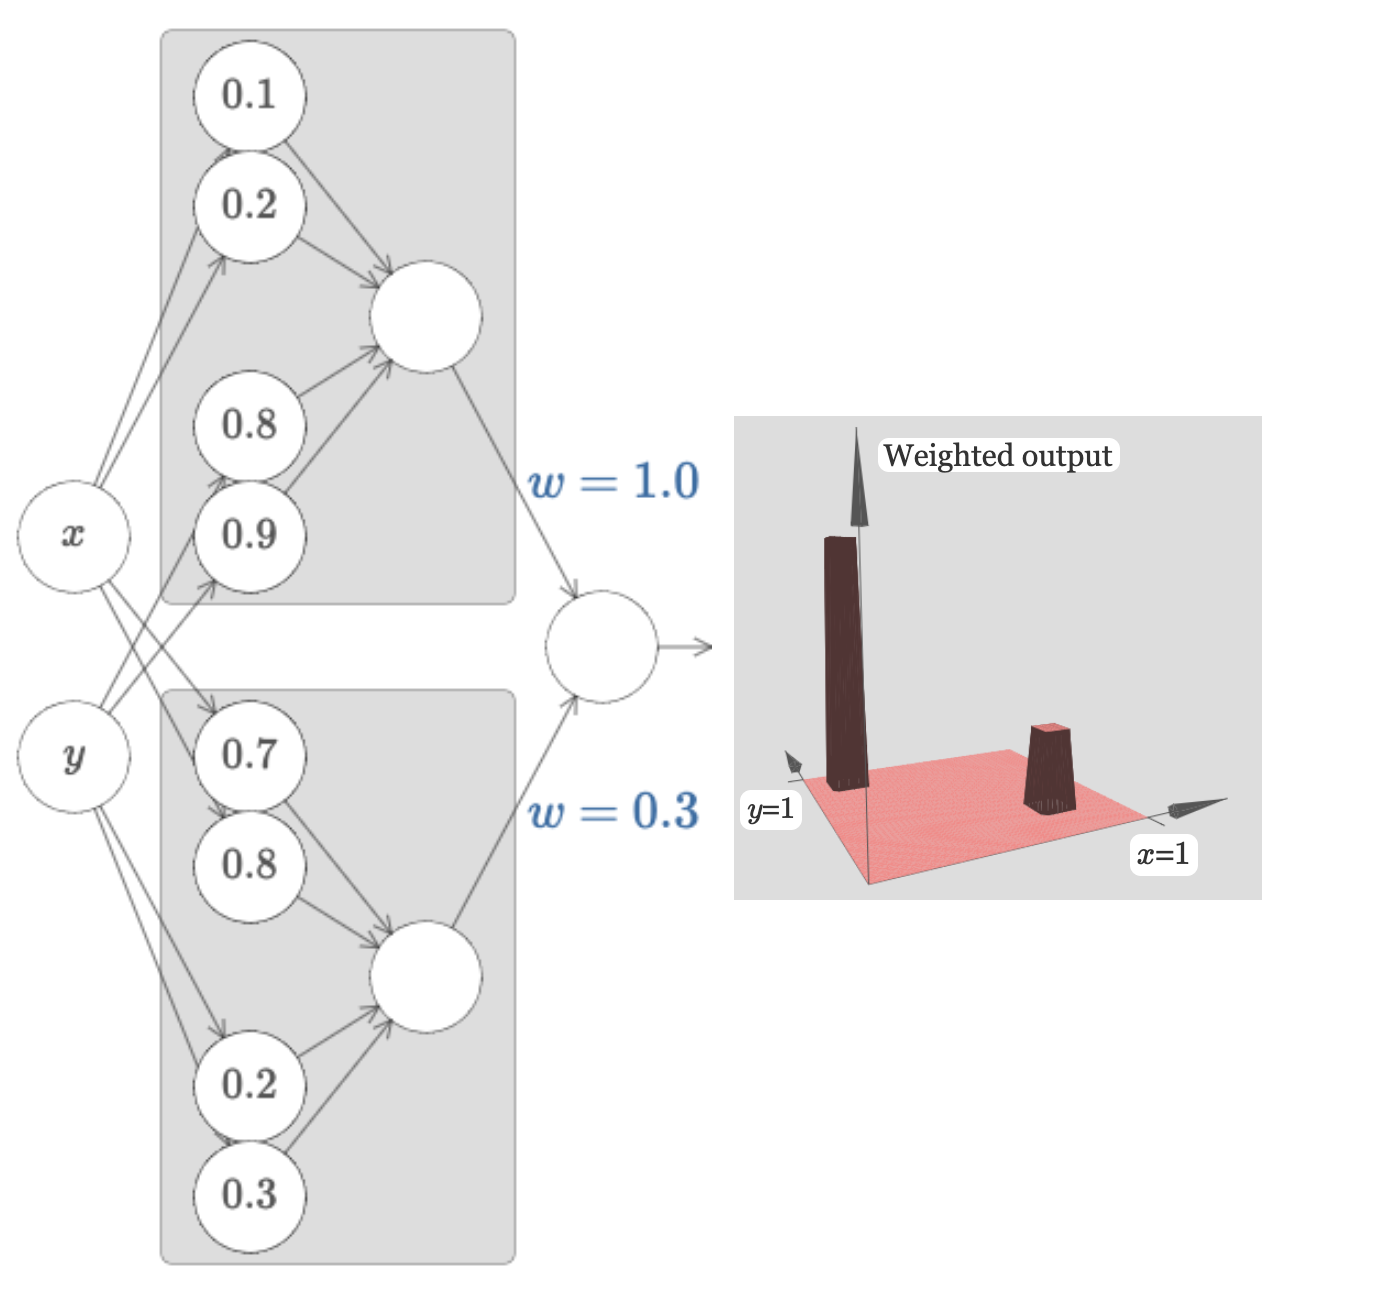
\includegraphics[scale=.35]{more-towers}
  
\end{frame}

%%%%%%%%%%%%%%%%%%%%%%%%%%%%%%%%%%%%%%%%%%%%%%%%%%%%%

\begin{frame}
  \frametitle{Many towers}
  
   \centering
  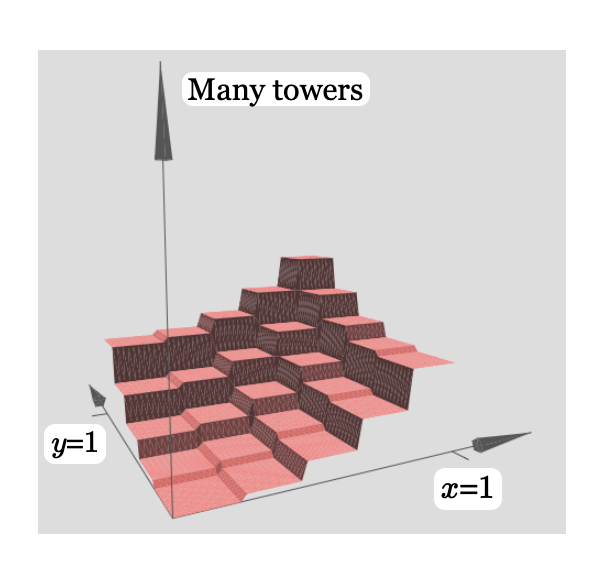
\includegraphics[scale=.35]{many-towers}
  
  \flushleft
  Once again, the shape of of the above should approximate $\sigma^{-1}(f)$, as all the plots we have seen before represent the weighted output in the last layer (not the net output).
  
\end{frame}

%%%%%%%%%%%%%%%%%%%%%%%%%%%%%%%%%%%%%%%%%%%%

\begin{frame}
  \frametitle{Even more input variables}
  
  Same reasoning, we try to compute multi-dimensional towers.
  
  The bias of the output neuron is then set to:
  
  \[ ( -m + \frac{1}{2} )h \quad \text{where $m$ is the number of inputs/dimensions} \]
  
\end{frame}


%%%%%%%%%%%%%%%%%%%%%%%%%%%%%%%%%%%%%%%%%%
\begin{frame}
  \frametitle{Final remarks}
  
  \begin{itemize}
  \item This just give an intuition of the universality of NN, does not say that it is the right way of learning functions;
  \item we have showed universality with more than one hidden layer, while the theorem says \tc{red}{one} hidden layer...
\item that does not mean it is in general a good idea to use only one layer (think of convolutional networks).
\end{itemize}
  
\end{frame}



%%%%%%%%%%%%%%%%%%%%%%%%%%%%%%%%%%%%%%%%%
\end{document}